\documentclass[11pt]{article}

\usepackage[margin=1in]{geometry}
\usepackage{amsmath}
\usepackage{amssymb}
\usepackage{booktabs}
\usepackage{caption}
\usepackage{enumitem}
\usepackage{float}
\usepackage{graphicx}
\usepackage{hyperref}
\usepackage{subcaption}
\usepackage{fvextra}

\hypersetup{
  colorlinks=true,
  linkcolor=blue,
  urlcolor=blue,
  citecolor=blue
}

\graphicspath{{../../results/selected_plots/sample_size/}}

\title{Sample-Size Simulation: Product-Mixture Probit Factors versus Joint-Mixture Gibbs}
\author{}
\date{\today}

\begin{document}
\maketitle

\section{Purpose}

This note documents the sample-size simulation used to compare two ways of fitting binary
probit factor-mixture structure in high-dimensional item-response data. The simulation was
designed to answer a practical question: when the latent factors have mixture structure, how
much data are needed for a full joint-mixture Gibbs sampler to recover the data-generating
parameters, and how does that compare with the proposed independent product-mixture fitting
strategy?

The comparison uses the same binary probit data-generating model for both methods, the same
post-processing alignment, and the same recovery metrics. Each Monte Carlo repetition simulates
a new dataset, including new latent mixture labels, factor values, probit noise, binary responses,
item intercepts, and loading matrices.

\section{Data-Generating Model}

For subject or model $i=1,\ldots,n$ and item $j=1,\ldots,p$, responses are generated through a
latent Gaussian probit variable,
\begin{align}
Z_{ij} &= \alpha_j + \lambda_j^\top f_i + \epsilon_{ij},
        \qquad \epsilon_{ij} \sim N(0,1), \\
X_{ij} &= \mathbf{1}\{Z_{ij} > 0\}.
\end{align}
The factor vector $f_i=(f_{i1},\ldots,f_{iH})^\top$ has independent marginal mixtures,
\begin{equation}
f_{ih} \sim \sum_{g=1}^G \pi_{hg} N(\mu_{hg}, \sigma_{hg}^2),
\qquad h=1,\ldots,H.
\end{equation}
Equivalently, the full $H$-dimensional factor distribution can be written as a joint Gaussian
mixture with $G^H$ profiles, where each profile corresponds to one Cartesian product of the
marginal component labels. This equivalence is important: the Gibbs comparator is correctly
specified as a joint mixture, while the proposed method exploits the product structure directly.

The simulation grid is:
\begin{itemize}[leftmargin=*]
  \item $H \in \{3,4\}$ latent factors;
  \item $G \in \{2,3\}$ mixture components per factor;
  \item $n \in \{100,500,1000,2000\}$ and $p=500$;
  \item 25 Monte Carlo repetitions per setting;
  \item IFEval-like item intercepts, with block structure plus random item-level variation;
  \item unequal mixture variances;
  \item two loading designs, labeled below as \textbf{Sparse} and \textbf{Cross}.
\end{itemize}

The Sparse loading design has one primary positive loading block per factor, with rare weak
positive cross-loadings. The Cross design keeps the same primary positive block structure but
adds more frequent signed cross-loadings. Figure~\ref{fig:dgp-lambda} shows representative
realizations of the DGP loading matrices for $H=4$. The actual simulation redraws $\Lambda$ in
each repetition; these figures are fixed-seed representative matrices generated by the same DGP
code.

\begin{figure}[H]
\centering
\begin{subfigure}{0.47\textwidth}
  \centering
  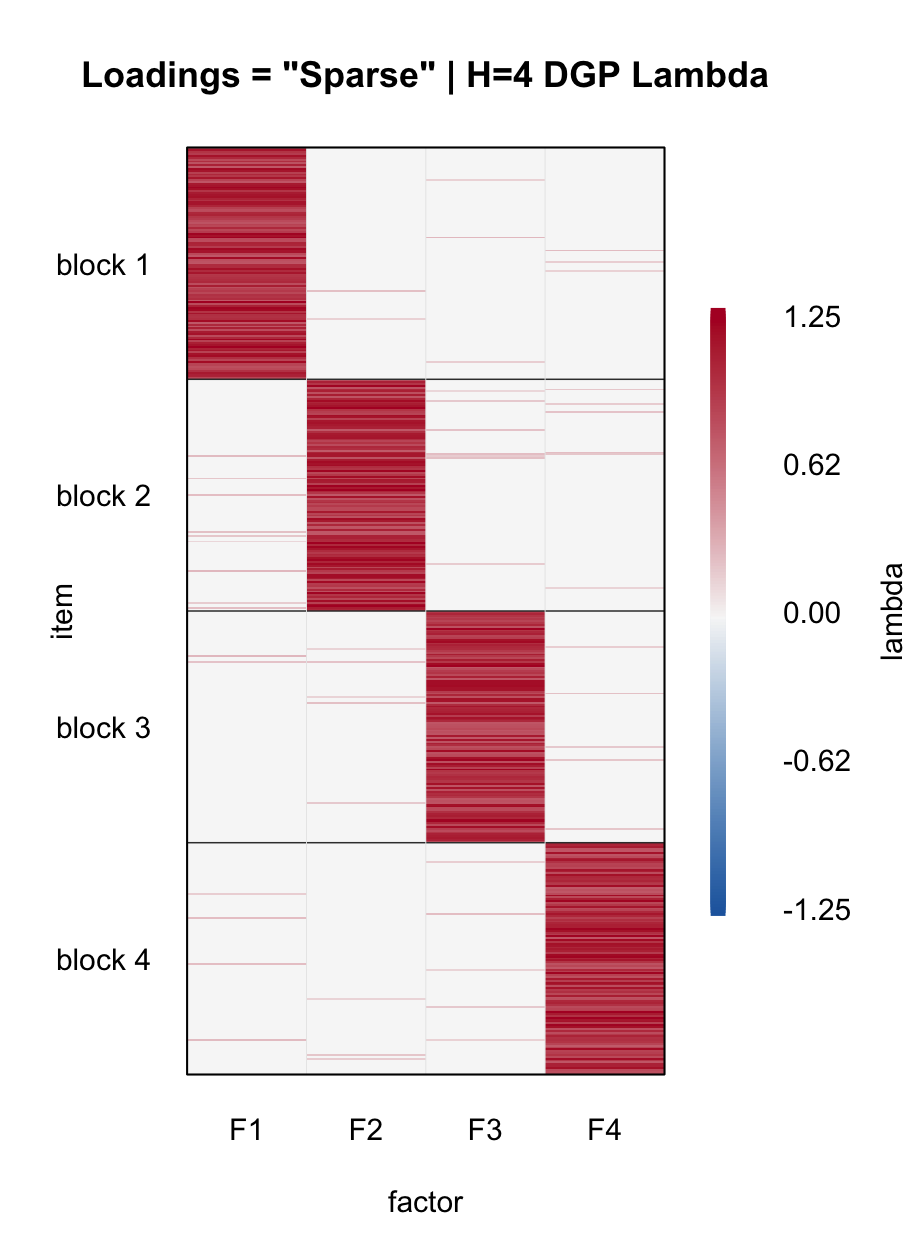
\includegraphics[width=\textwidth]{dgp_lambda_heatmap_sparse_H4.png}
  \caption{Sparse loading design.}
\end{subfigure}
\hfill
\begin{subfigure}{0.47\textwidth}
  \centering
  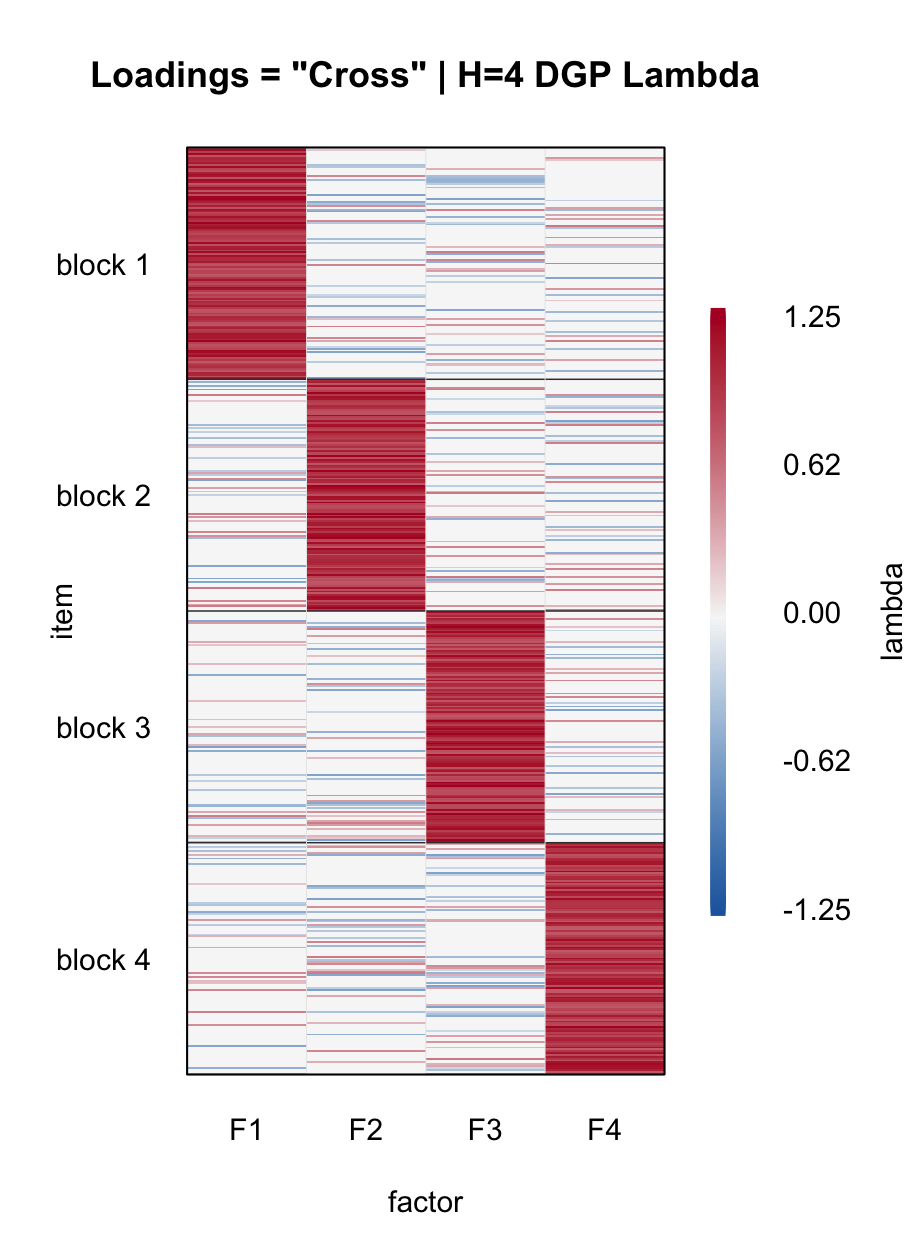
\includegraphics[width=\textwidth]{dgp_lambda_heatmap_cross_H4.png}
  \caption{Cross loading design.}
\end{subfigure}
\caption{Representative DGP loading matrices for $H=4$ and $p=500$.}
\label{fig:dgp-lambda}
\end{figure}

\section{Methods Compared}

\subsection{Proposed Product-Mixture Probit Factor Method}

The proposed method fits the independent marginal-mixture factor model directly. The fitted model
is
\begin{align}
X_{ij} \mid f_i,\alpha_j,\lambda_j
  &\sim \mathrm{Bernoulli}\{\Phi(\alpha_j+\lambda_j^\top f_i)\}, \\
f_{ih} &\sim \sum_{g=1}^{G} \pi_{hg} N(\mu_{hg},\sigma_{hg}^2),
        \qquad h=1,\ldots,H,
\end{align}
with independent factor coordinates. The algorithm has two stages.

\paragraph{Stage 1: augmented-probit spectral pretraining.}
The binary responses are augmented with latent probit variables $Z_{ij}$ drawn or updated from
their truncated normal conditional distribution. The current $Z$ matrix is centered and a rank
$H$ singular value decomposition is used to initialize factor scores. The resulting spectral
scores are rotated so that each coordinate is well described by a one-dimensional Gaussian
mixture. In this simulation the rank is treated as known and the pretraining stage runs for at
most 10 augmentation/rotation iterations.

\paragraph{Stage 2: MAP refinement.}
Starting from the pretrained factors and loadings, the algorithm alternates among:
\begin{enumerate}[leftmargin=*]
  \item updating augmented probit variables or their conditional expectations;
  \item updating item intercepts and sparse loadings through probit surrogate regressions;
  \item updating factor scores under the current loading/intercept values;
  \item updating each marginal mixture distribution by MAP mixture updates;
  \item normalizing factor scale so the probit linear predictor is unchanged while factor
        mixture means and variances remain comparable across iterations.
\end{enumerate}
The refinement stage also runs for at most 10 iterations. The loading penalty and mixture MAP
priors are fixed across the simulation grid.

\subsection{Joint-Mixture Factor Gibbs Comparator}

The comparator is a correctly specified joint-mixture factor model. Instead of representing the
factor distribution as $H$ independent $G$-component mixtures, it represents the factor vector as
a single mixture with $K=G^H$ joint profiles:
\begin{align}
f_i \mid c_i=k &\sim N_H(\mu_k,\mathrm{diag}(\sigma_{k1}^2,\ldots,\sigma_{kH}^2)), \\
\Pr(c_i=k) &= \omega_k, \qquad k=1,\ldots,G^H, \\
X_{ij} \mid f_i,\alpha_j,\lambda_j
  &\sim \mathrm{Bernoulli}\{\Phi(\alpha_j+\lambda_j^\top f_i)\}.
\end{align}
This model is correctly specified for the simulated data because the Cartesian product of the
independent marginal mixtures induces exactly such a joint mixture.

The Gibbs sampler uses probit augmentation and cycles through:
\begin{enumerate}[leftmargin=*]
  \item sampling $Z_{ij}$ from its truncated normal full conditional given $X_{ij}$;
  \item sampling or updating item intercepts and loadings conditional on $Z$ and factor scores;
  \item sampling factor scores $f_i$ conditional on $Z$, loadings, intercepts, and class labels;
  \item sampling joint profile labels $c_i$;
  \item updating joint mixture weights, means, and diagonal variances;
  \item applying the same scale normalization convention used for the proposed method.
\end{enumerate}
Each Gibbs fit uses 2000 iterations, with 1000 burn-in iterations and no thinning.

\section{Alignment and Evaluation}

Factor models are unidentified up to signed permutations of the latent coordinates. To make the
comparison apples-to-apples, both methods use the same post-processing strategy: choose the
factor permutation and sign pattern that best aligns the estimated loading matrix with the true
DGP loading matrix. The same alignment is then applied to factor scores and mixture parameters.

The plotted recovery metrics summarize:
\begin{itemize}[leftmargin=*]
  \item RMSE for item intercepts $\alpha$;
  \item RMSE for loadings $\Lambda$;
  \item RMSE for mixture means;
  \item RMSE for mixture variances;
  \item RMSE for joint-profile mixture weights, computed by vectorizing the aligned $G^H$
        profile probabilities;
  \item flattened factor-score correlation after alignment.
\end{itemize}
Each point in the recovery plots is the mean across 25 repetitions. Error bars show plus/minus
two Monte Carlo standard deviations. Runtime plots report mean $\log(\mathrm{seconds})$ with
plus/minus two standard deviations; the raw timing field is total elapsed wall-clock time for the
full method fit.

\section{Results Summarized}

Across the 32 combinations of loading design, $H$, $G$, and sample size, the proposed product
mixture has lower mean RMSE than the joint Gibbs comparator for loadings, mixture means, mixture
variances, and mixture weights. It also has higher mean flattened factor-score correlation in all
32 cells. At $n=2000$, loading RMSE is close for $G=2$ but the joint Gibbs sampler remains much
less accurate for mixture means, variances, and profile weights, especially when $G=3$ and
$K=G^H$ is large.

The main interpretation is computational and statistical. Although the joint-mixture Gibbs model
is correctly specified, it must estimate $G^H$ joint profiles. This creates many mixture
parameters and a hard class-allocation problem in the same $n,p$ regimes where the product
mixture only estimates $H$ separate one-dimensional mixtures. The product-mixture method exploits
the factorial structure, so it recovers the relevant factor axes and marginal mixture parameters
with substantially less apparent sample-size burden.

Figures~\ref{fig:recovery-h4g3-sparse}--\ref{fig:timing-h4g3} show the most difficult setting,
$H=4,G=3$, where the joint mixture has $3^4=81$ profiles. The full set of selected plots for all
settings is stored in the repository under the selected sample-size plot directory.

\begin{figure}[H]
\centering
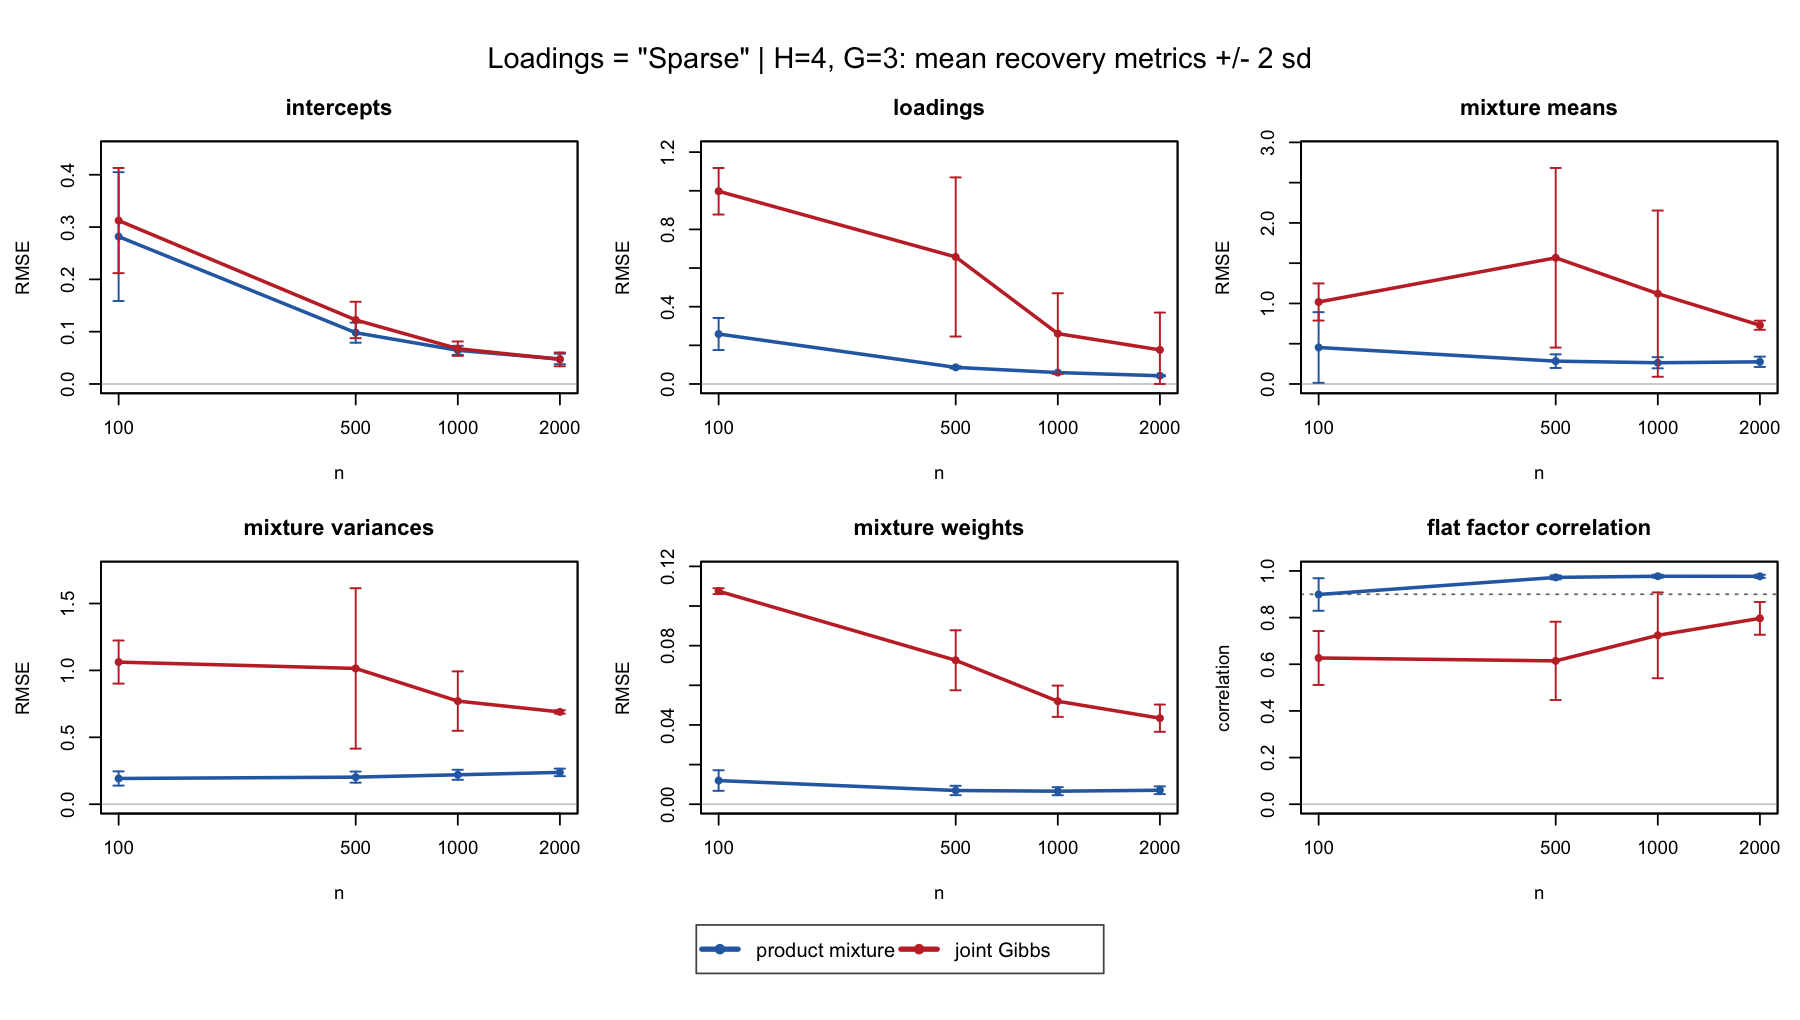
\includegraphics[width=0.92\textwidth]{checkpoint_parameter_recovery_panel_balanced_moderate_few_positive_cross_H4_G3.png}
\caption{Parameter recovery in the $H=4,G=3$ setting with Sparse loadings. Lower is better for RMSE panels; higher is better for factor correlation.}
\label{fig:recovery-h4g3-sparse}
\end{figure}

\begin{figure}[H]
\centering
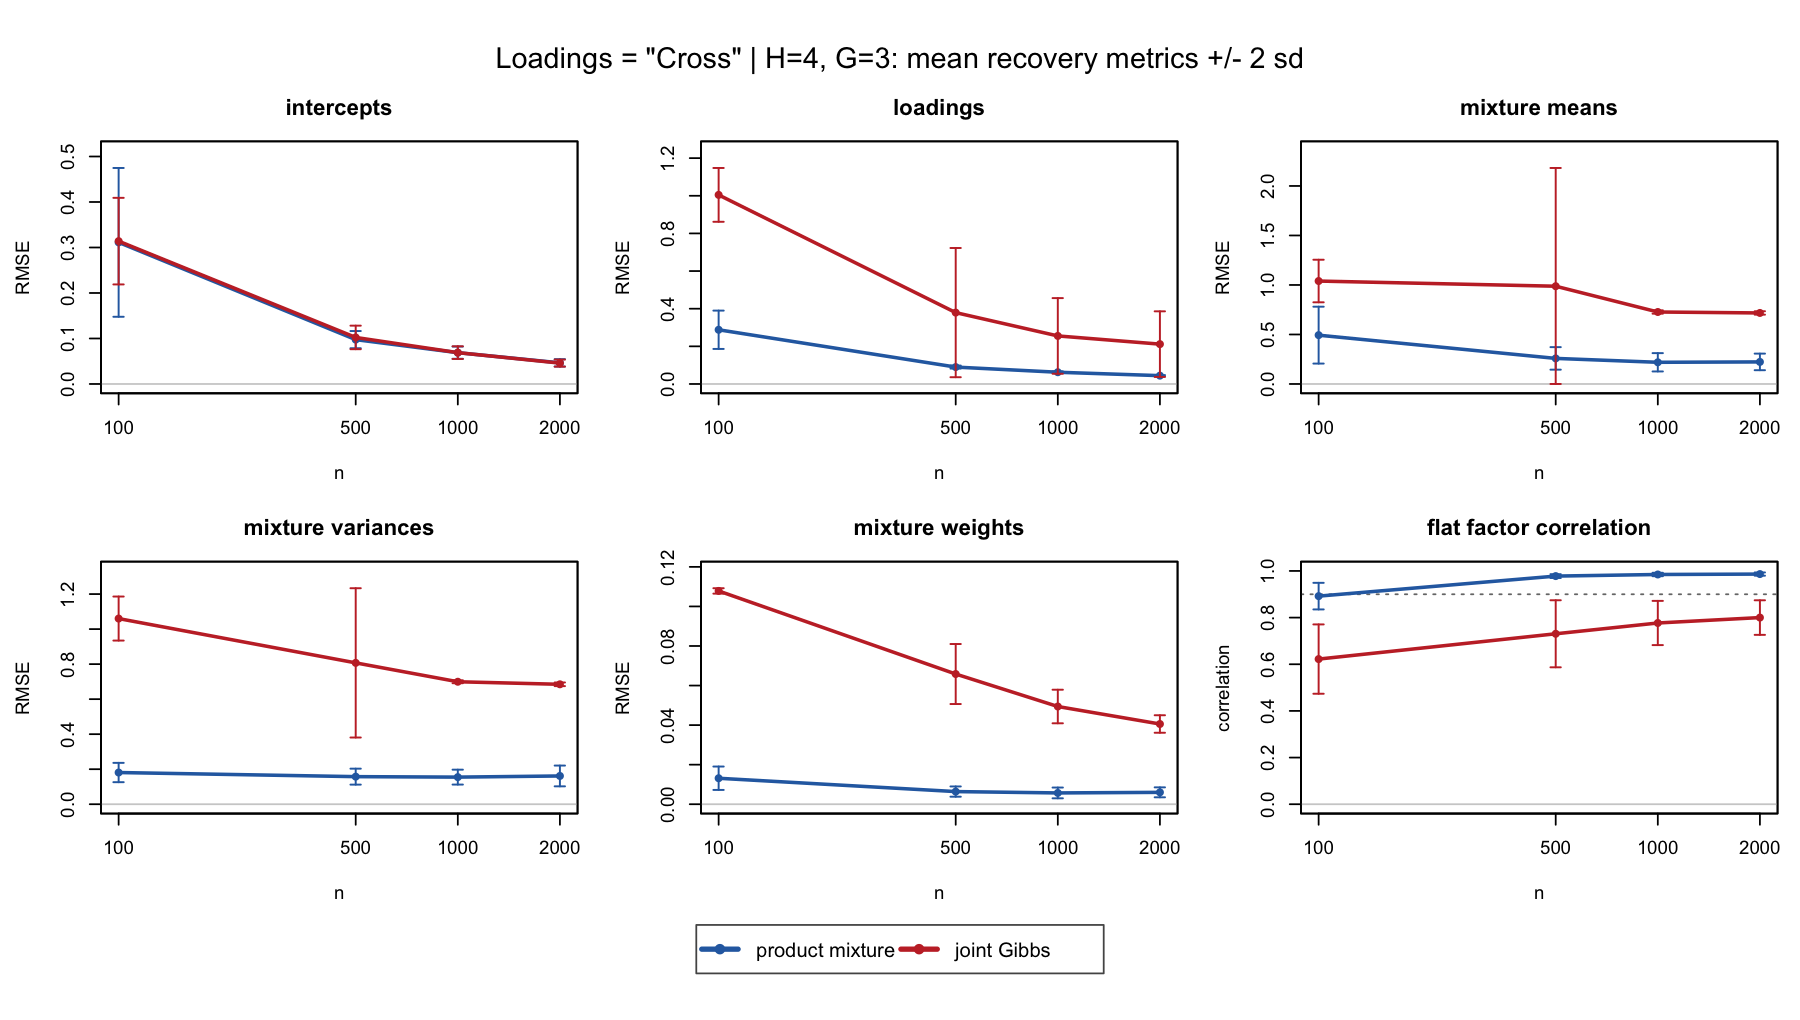
\includegraphics[width=0.92\textwidth]{checkpoint_parameter_recovery_panel_balanced_moderate_dense_signed_cross_H4_G3.png}
\caption{Parameter recovery in the $H=4,G=3$ setting with Cross loadings. Lower is better for RMSE panels; higher is better for factor correlation.}
\label{fig:recovery-h4g3-cross}
\end{figure}

\begin{figure}[H]
\centering
\begin{subfigure}{0.49\textwidth}
  \centering
  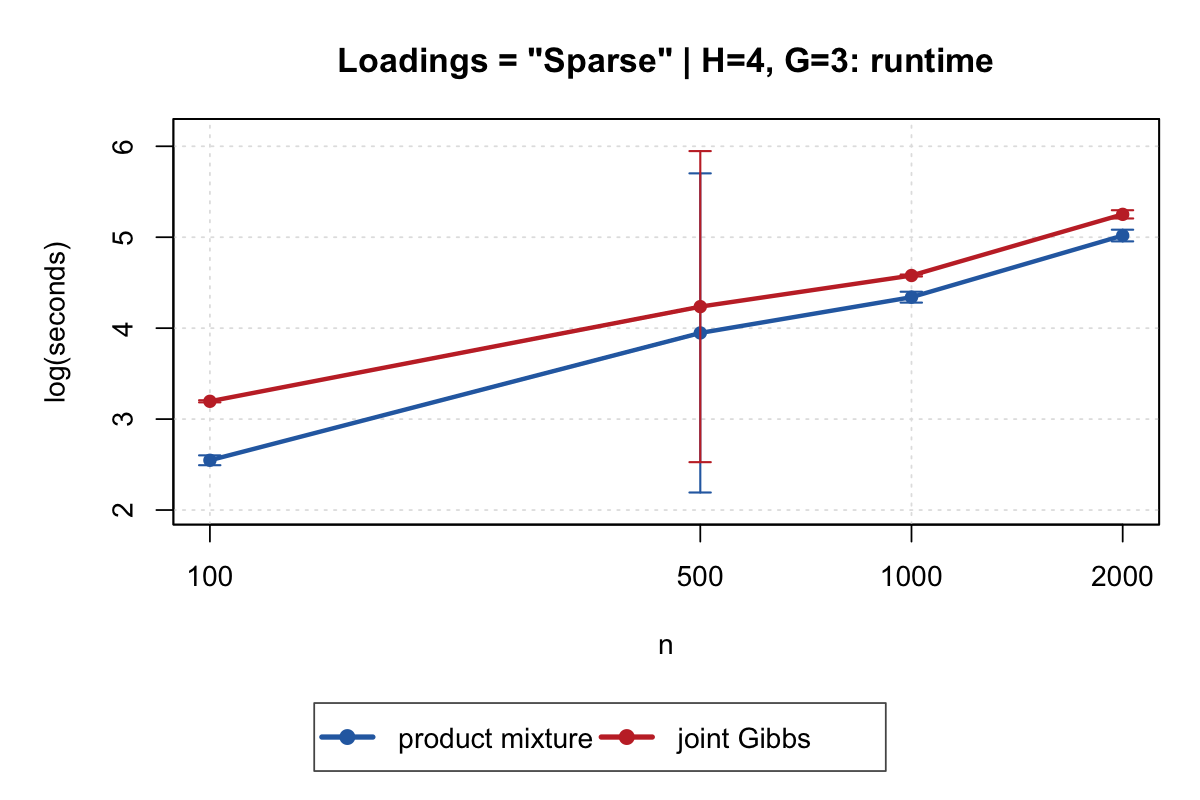
\includegraphics[width=\textwidth]{checkpoint_timing_log_seconds_balanced_moderate_few_positive_cross_H4_G3.png}
  \caption{Sparse loadings.}
\end{subfigure}
\hfill
\begin{subfigure}{0.49\textwidth}
  \centering
  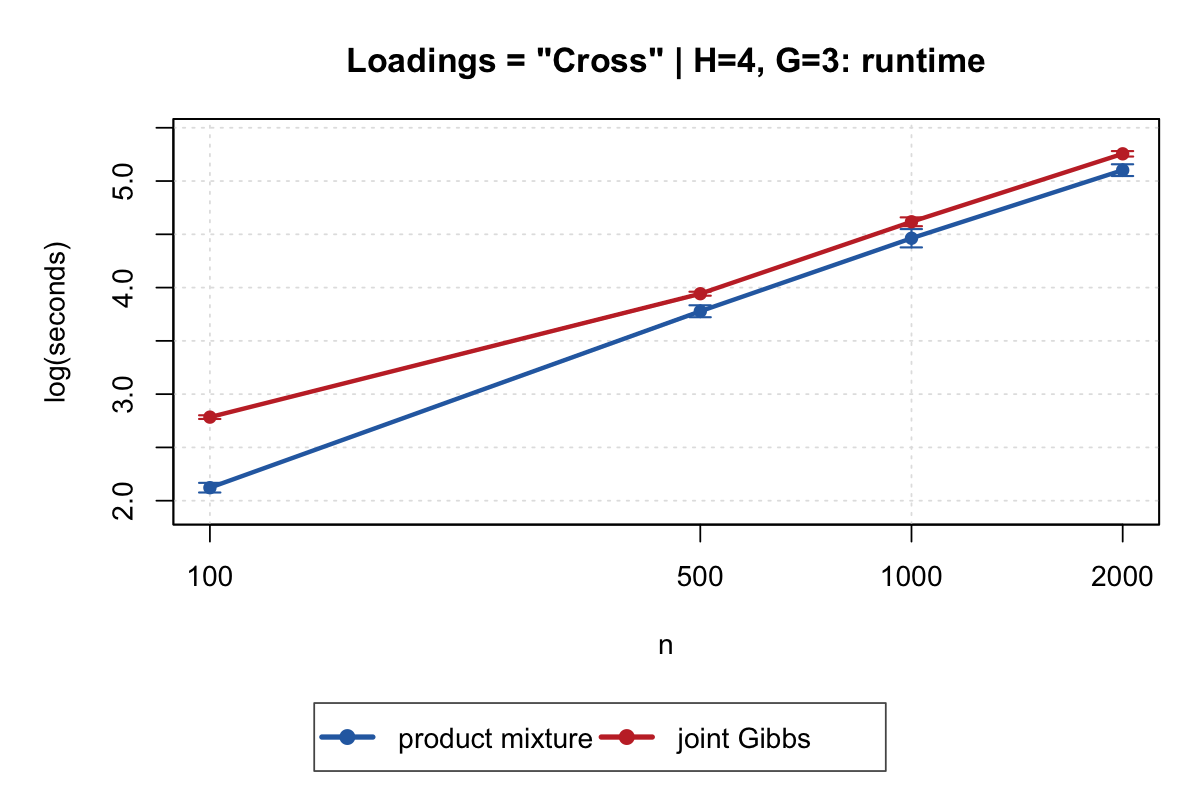
\includegraphics[width=\textwidth]{checkpoint_timing_log_seconds_balanced_moderate_dense_signed_cross_H4_G3.png}
  \caption{Cross loadings.}
\end{subfigure}
\caption{Runtime summaries in the $H=4,G=3$ setting. The y-axis is $\log(\mathrm{seconds})$.}
\label{fig:timing-h4g3}
\end{figure}

\section{Reproducibility}

The main simulation is launched with:
\begin{Verbatim}[breaklines=true,fontsize=\small]
Rscript scripts/sample_size/run_sampledZ_full_pgrid_smallp_gibbs_MAP_intercepts.R
\end{Verbatim}
The paper-facing figures are regenerated from the completed checkpoint by setting
\texttt{OUT\_DIR} to the full sample-size output directory and running:
\begin{Verbatim}[breaklines=true,fontsize=\small]
Rscript scripts/sample_size/plot_dgp_loading_heatmaps.R
Rscript scripts/sample_size/plot_sample_size_rmse_panels.R
Rscript scripts/sample_size/plot_sample_size_timing_lines.R
\end{Verbatim}
The selected summary tables used to audit these results are:
\begin{itemize}[leftmargin=*]
  \item \texttt{results/selected\_tables/sample\_size/checkpoint\_parameter\_recovery\_summary.csv};
  \item \texttt{results/selected\_tables/sample\_size/checkpoint\_timing\_log\_seconds\_summary.csv};
  \item \texttt{results/selected\_tables/sample\_size/dgp\_lambda\_matrix\_*.csv}.
\end{itemize}

\end{document}
